%-----------------------
% Title page
%-----------------------
\begin{titlepage}
  \centering

  \textsc{ELEC4630 Assignment 3}\\
  \vspace{9cm}

  \rule{\linewidth}{0.5pt}\\

  \vspace{1em}
  \LARGE\textsc{Question 2}\\
  \vspace{1em}

  \LARGE\uppercase{\textbf{{Animal Image Classification}}}\\

  \rule{\linewidth}{2pt}\\

  \vfill

  \normalsize{Deren Teo (45285545)}
  \vspace{1cm}

\end{titlepage}

%-----------------------
% Report body
%-----------------------
\section{Introduction}

Image classification is the task of having a computer assign labels to or categorize an image based on the objects present within it. This has innumerable practical applications in all fields, especially with the increasing demand for intelligent and autonomous systems. However, until the advent of convolutional neural networks (CNNs) in 1998 with the introduction of LeNet (LeNet-5), no system was able to perform the task with any reasonable accuracy \cite{amidi_2017}. Though image classification systems have since improved considerably, until relatively recently, variants of the CNN architecture remained the state-of-the-art for image classification \cite{paperswithcode_2023}. This report explores the capabilities of a popular CNN, ResNet-18, by fine-tuning a model pre-trained on ImageNet \cite{stanfordvisionlab_2020} to classify ten different animals.

\section{Background Theory}

\subsection{Convolutional Neural Networks}

As a neural network, convolutional neural networks (CNNs) consist of an input layer, output layer, and multiple hidden layers in between \cite{mathworks_2017}. Figure \ref{fig:convnet} presents an example of a typical CNN architecture from \cite{mathworks_2017}.

\begin{figure}[ht]
  \centering
  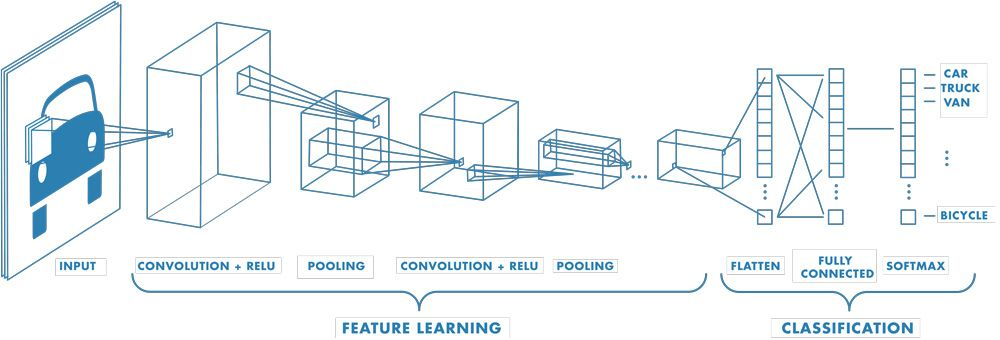
\includegraphics[width=\textwidth]{images/q2_convnet.jpg}
  \caption{Example of a typical CNN architecture \cite{mathworks_2017}.}
  \label{fig:convnet}
\end{figure}

Figure \ref{fig:convnet} illustrates that an image is input to the CNN and a label, or classification, is output. In between, CNNs consist of three main types of layers: convolutional, pooling and fully-connected \cite{ibm_2020}.

The convolutional layer is the namesake of the architecture, and performs the majority of the computation done by the network \cite{ibm_2020}. In a convolutional layer, input data is convolved with a kernel to produce a feature map \cite{ibm_2020}. For the first layer in a CNN, the input data is the image itself; this may be a matrix in the case of a single-channel image, or a 3D tensor for a three-channel image. For subsequent convolutional layers, the input data is the output of a previous convolutional or pooling layer. The kernel is typically a 3D tensor of height and width 3x3 pixels \cite{ibm_2020}, and depth equal to the depth of the input data. The kernel is applied to an area of the input data using a dot product operation, which produces an output value \cite{ibm_2020}. The kernel is then shifted one or more pixels across the image and the process repeats until the kernel has covered the entire image \cite{ibm_2020}. The set of outputs then creates a feature map \cite{ibm_2020}, whose purpose is to identify various features such as colours and geometries. Finally, a non-linear activation function is applied to the feature map to introduce non-linearity; this is a requirement for the model to solve non-linear problems. The most common activation function is the Rectified Linear Unit (ReLU) \cite{ibm_2020}, which maps negative values to zero.

Typically, the earlier convolutional layers recognise simpler features, such as colours and edges \cite{ibm_2020}. Subsequent layers recognise increasingly complex features as combinations of simpler features, until an object of classification interest is recognised \cite{ibm_2020}.

The pooling layer exists to reduce the dimensionality of a convolutional output, which reduces the complexity of subsequent layers and therefore decreases the model training time \cite{ibm_2020}. Pooling occurs similarly to convolution but without any kernel weights \cite{ibm_2020}. Instead, the pooling kernel simply aggregates the values underneath it, typically either by selecting the maximum or average value \cite{ibm_2020}. Selecting the maximum value, known as max pooling, is more common \cite{ibm_2020}. While pooling is common in CNNs, some networks do not have pooling layers \cite{springenberg_2014}. Furthermore, some authors even suggest the pooling layer to be detrimental to performance \cite{sunkara_2023}.

The last few layers of a CNN are typically fully-connected layers, which perform classification based on the features extracted by the convolutional layers \cite{ibm_2020}. A fully-connected layer is what is typically presented in illustrations of neural networks, where each node (or ``neuron'') is connected to every node in the previous layer \cite{ibm_2020}. Rather than a ReLU activation function, the softmax function tends to be more suitable for the fully-connected layers \cite{ibm_2020}. The softmax function pushes output values towards either zero or one, which is suitable for producing classification probabilities \cite{ibm_2020}.

\subsection{ResNet-18}

The model of focus in this report is ResNet-18, a residual neural network (ResNet) based on the CNN architecture \cite{he_2016}. Compared to vanilla CNNs, ResNets introduce ``shortcut connections'' between model layers \cite{he_2016}. While the theoretical foundation of this modification lies outside the scope of this report, there is empirical evidence that ResNets are easier to optimise and achieve better results than vanilla CNNs with a similar number of parameters \cite{he_2016}.

Figure \ref{fig:resnet18} presents the architecture of the ResNet-18 model, an 18-layer ResNet, from \cite{ramzan_2019}.

\begin{figure}[ht]
  \centering
  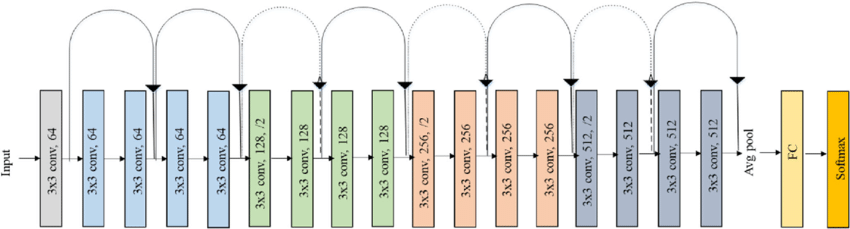
\includegraphics[width=\textwidth]{images/q2_resnet18.png}
  \caption{ResNet-18 architecture \cite{ramzan_2019}}
  \label{fig:resnet18}
\end{figure}

The notable features visible in Figure \ref{fig:resnet18} are the shortcut connections and lack of pooling between convolutional layers. ResNet-18 is originally trained on the ImageNet 2012 classification dataset \cite{russakovsky_2015} of 1.28 million training images split between 1000 classes \cite{he_2016}. To suit the ImageNet classification task, the input layer has dimensions 224$\times$224 in three channels, and the final classification is accomplished by a 1000-way fully-connected layer with softmax activation \cite{he_2016}.

The original ResNet-18 model achieved 72.12\% accuracy on the ImageNet validation set of 50k images \cite{he_2016}. Larger ResNet models of up to 152 layers were also evaluated in the seminal paper, with performance corresponding to size \cite{he_2016}. At the time of introduction, ResNet-152 achieved state-of-the-art results on ImageNet with 80.62\% validation accuracy \cite{he_2016}.

\subsection{Transfer Learning}

Transfer learning is a machine learning technique where a model trained on a more generic task is fine-tuned to perform a more specific task \cite{brownlee_2019}. The utility of transfer learning is in leveraging a pre-trained model to reduce the time and compute requirement for a different machine learning task \cite{brownlee_2019}. For example, training of the original ResNet-18 model on the ImageNet data set required 3.5 days, even after extensive optimisation and parallelisation across four GPUs \cite{gross_2016}. However, once trained, the model can easily be fine-tuned for specific image classification tasks even within seconds and achieve a reasonable accuracy \cite{howard_2020}.

There are two predominant scenarios for transfer learning: using a pre-trained model as fixed feature extractor, or fine-tuning the pre-trained model \cite{stanforduniversity_2023}. For the first, the fully-connected classification layer of a pre-trained network is replaced with one specific to a different task \cite{stanforduniversity_2023}. The pre-trained network is used as a feature extractor and is fixed; only the new classifier is trained \cite{stanforduniversity_2023}. For the second scenario, parts of the pre-trained model, or the entire model, are re-trained for a different task \cite{stanforduniversity_2023}. This approach may or may not involve replacing the classification layer \cite{stanforduniversity_2023}. How much of the model is re-trained often depends on the similarity of the new classification task to the original training data \cite{stanforduniversity_2023}. Layers in a CNN become progressively more specific from input to output; therefore, later layers are more specific to the original training data \cite{stanforduniversity_2023}. The second approach is adopted in the methodology presented in this report.

\section{Methodology}

This section describes the approach used to fine-tune a ResNet-18 model to classify ten different animals. These animals are: lions, elephants, tigers, giraffes, bears, wolves, dolphins, penguins, eagles, and kangaroos.

The methodology is an extension of the examples provided by fastai in \cite{howard_2022} and \cite{howard_2020}. It is based on the fastai and PyTorch libraries for Python. The methodology will use the PyTorch implementation of ResNet-18 with pre-trained weights \cite{torchcontributors_nd}. The model with pre-trained weights closely reproduces the results of the original paper \cite{he_2016} on the ImageNet data set \cite{torchcontributors_nd}.

\subsection{Data Retrieval}

A data set of images of each animal is constructed by querying the DuckDuckGo API. The Python notebook implementation can be viewed in Appendix \ref{app:classifying_animals_ipynb}. In summary:

\begin{enumerate}
  \item The program creates a directory for the first animal (lion). Or, if a directory already exists, it is assumed the data has been previously downloaded and the animal is skipped.

  \item The \texttt{duckduckgo\_search} library \cite{deedy5_2023} is used to download 100 images of the animal by querying the term, e.g. ``lion animal'', and downloading the first 100 image results.

  \item Steps 1 and 2 are repeated for each animal, which can be programatically automated using a loop statement over a list of animal names.

  \item The images are checked using the \texttt{fastai} library and broken or unsuccessful downloads are removed. This typically results in between 90 to 100 images of each animal.

  \item The images are manually perused using a file explorer, to ensure each search term returned appropriate results, and not a misinterpretation of the search term.

  \item The first 20 images of each animal are manually separated into a ``test'' directory, with the remaining images becoming the training data set.

\end{enumerate}

\subsection{Model Training}

As mentioned, a pre-trained ResNet-18 model provided by PyTorch is fine-tuned for the new data set of animals. This is made simple by the fastai API. The steps are:

\begin{enumerate}
  \item A \texttt{DataBlock} is created to load the training data. This is a fastai abstraction of a data pipeline, and is configured with the following:
  \begin{itemize}
    \item the model input is specified as images and the output as categories (or classes);
    \item a validation split of 20\% is specified, to be randomly selected from the data; and
    \item the images are to be resized to a maximum dimension of 192 pixels by ``squishing''.
  \end{itemize}

  \item A pre-trained ResNet-18 model is downloaded from PyTorch and associated with the data pipeline. The model is specified to use error rate as a validation metric.

  \item The model is fine-tuned over three epochs. Or, a previously saved model can be loaded.

  \item The tuned model can be saved to avoid re-training whenever the notebook is reloaded:
  \begin{center}
    \texttt{learn.save(file=`resnet18-animal-tuned')}
  \end{center}
  The saved model can be loaded in place of Step 3 using:
  \begin{center}
    \texttt{learn.load(`resnet18-animal-tuned')}
  \end{center}

\end{enumerate}
\vspace{1em}

Figure \ref{fig:dls_batch} shows a sample of training images input to the model by the data pipeline.

\begin{figure}[ht]
  \centering
  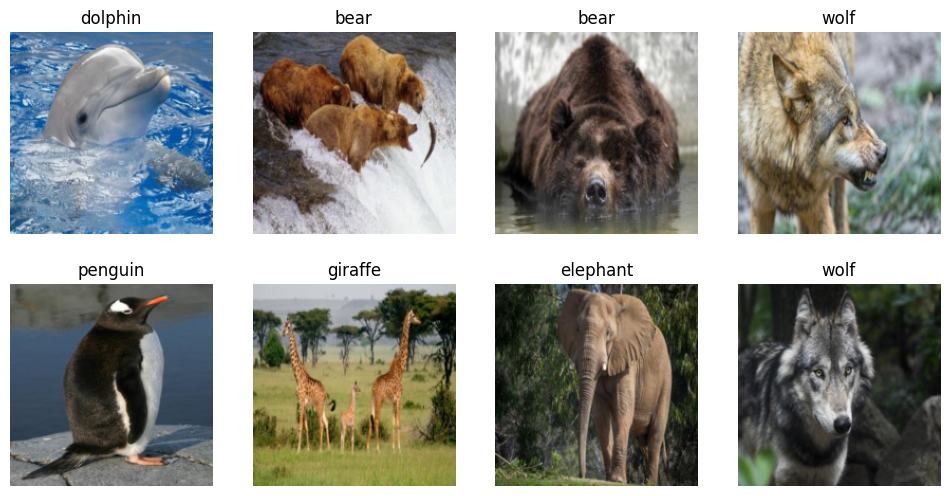
\includegraphics[width=0.9\textwidth]{images/q2_dls_batch.png}
  \caption{Sample of images output by the \texttt{DataBlock} pipeline.}
  \label{fig:dls_batch}
\end{figure}

During the fine-tuning step, the model should print statistics after each epoch: training loss, validation loss and error rate. Ideally, each statistic decreases after every epoch; however, due to the stochastic nature of deep learning, this may not necessarily occur. Regardless, the final training loss, validation loss and error rate should all be very low. In particular, an error rate of 2\% or less is common, which corresponds to an accuracy on the validation set of 98\% or greater.

Although the validation loss is a reasonable indication of model performance, it is best practice to evaluate the model on data completely withheld from the training process. This avoids bias in the performance result from testing the model on data which influenced the model tuning, and is the purpose of the separate testing set of 20 images per animal.

\subsection{Model Evaluation}

Finally, the model performance is evaluated on the withheld test set, as follows:

\begin{enumerate}
  \item A new data loader for the test data is created and specified as labelled, which is not the default asumption for test data in fastai.

  \item The fine-tuned model is used to make predictions on the test data. If the data is specified as labelled, these are returned alongside the model predictions.

  \item The model accuracy is calculated by comparing the predictions and labels. The percentage accuracy and total number of correct prediction is printed to the console.

\end{enumerate}

\section{Results}

The result of the model performance evaluation on the test set is printed as:

\begin{center}
  \texttt{Test accuracy: 100.00\% (200/200)}
\end{center}

The model made no errors on the test set, which makes redundant visualising a confusion matrix for the test result. However, the fine-tuning process leading up to this test result did not finish with 100\% validation accuracy. Therefore, Figure \ref{fig:validation_confusion} instead presents a confusion matrix for the validation result after the final fine-tuning epoch. This shows a single misclassification, which is visualised in Figure \ref{fig:validation_top_loss}.

\begin{figure}[ht]
  \centering
  \begin{subfigure}[t]{0.45\textwidth}
    \vskip 0pt % provide baseline to top-align subfigures
    \centering
    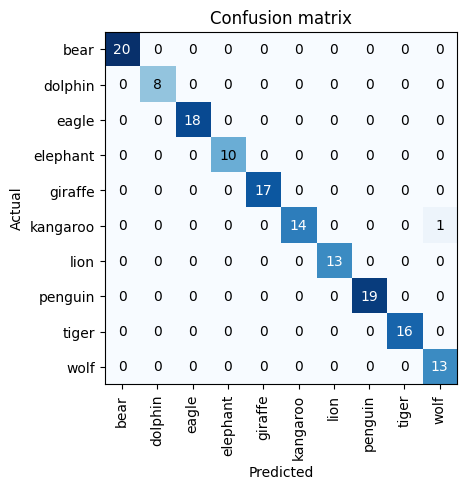
\includegraphics[width=\textwidth]{images/q2_validation_confusion.png}
    \caption{Confusion matrix}
    \label{fig:validation_confusion}
  \end{subfigure}
  \hfill
  \begin{subfigure}[t]{0.45\textwidth}
    \vskip 0pt % provide baseline to top-align subfigures
    \centering
    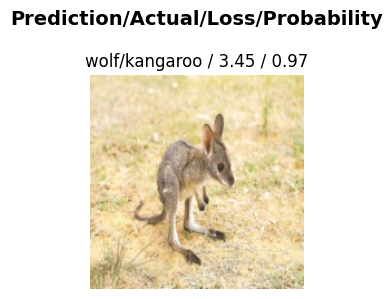
\includegraphics[width=\textwidth]{images/q2_validation_top_loss.png}
    \caption{Highest loss}
    \label{fig:validation_top_loss}
  \end{subfigure}
  \caption{Confusion matrix and highest loss validation result after final fine-tuning epoch.}
\end{figure}

The columns of the confusion matrix represent the classifications by the model, and the rows represent the true classifications according to which animal search term returned the result. The numbers along the diagonal represent correct classifications, whereas the numbers off the diagonal indicate which classes were confused and how often for incorrect classifcations.

Therefore, it is evident that one kangaroo image in the validation set is misclassified as a wolf.

\newpage
\section{Discussion}

This report has presented a method of classifying images of ten different animals by fine-tuning a pre-trained deep neural network. The network, ResNet-18, is fine-tuned on a training set of approximately 800 images and tested on a separate set of 200 images. The classifier achieves 100\% accuracy on the test set, though makes a single misclassification on the validation set in the final training epoch.

Figure \ref{fig:validation_top_loss} presents the single misclassified image. The image pictures a juvenile kangaroo, but is misclassified as a wolf. A brief perusal of the training data finds that the image is the only representation of a juvenile kangaroo without an adult kangaroo also in the same frame. Possibly due to both the colouration and hunched stature of the juvenile kangaroo, the latter of which is uncommon among other kangaroos in the training images, the model predicts with high probability (0.97) that the image contains a wolf. The resulting loss is therefore very high (3.45). Interestingly, if the model is repeatedly re-trained, this single misclassification is common, but does not always occur. Sometimes, the model fine-tunes to 100\% validation accuracy. This reflects the stochastic nature of neural networks and the resulting importance of sufficient training data and multiple trials.

To gain an intuition into how the tuned model differentiates the various animal classes, and why certain examples may be confused, it can help to visualise the representations of the training data in the model feature space. This is a non-trivial task because deep neural networks operate in very high-dimensional feature spaces. Dimensionality reduction can be applied to project the high-dimensional representation into a lower dimension for visualisation purposes, with the obvious caveat that some variance is undoubtedly lost in doing so.

For example, Figure \ref{fig:tsne} presents the representation of the training data in the feature space of the final feature-extraction layer of the fine-tuned ResNet-18 model, projected into 2D.

\begin{figure}[ht]
  \centering
  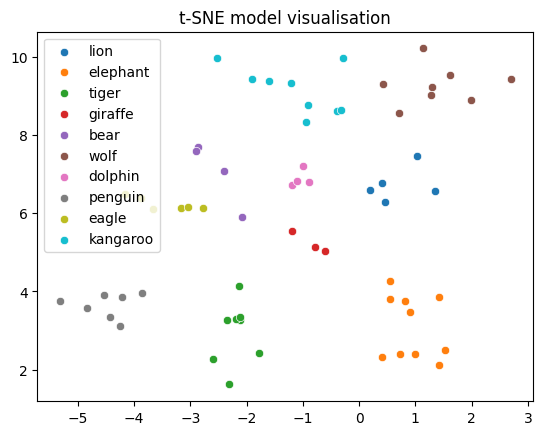
\includegraphics[width=0.6\textwidth]{images/q2_tsne.png}
  \caption{Training data represented by final feature-extraction layer, projected in 2D.}
  \label{fig:tsne}
\end{figure}

The dimensionality reduction technique applied to obtain the above is t-SNE (t-distribution stochastic neighbour embedding). t-SNE aims to preserve relative distances in the higher-dimensional space when projecting into a lower dimension \cite{serebryakov_2020}. The distance between points in the lower-dimensional space is tuned to minimize the difference between the relative distances in the higher-dimensional space, with distance measured using Kullback-Leibler divergence \cite{serebryakov_2020}.

Some classes are distinctly separated from the rest, notably penguins and tigers. This is semantically meaninful, as these animals have distintive colourations compared to the other classes. Meanwhile, the distributions of wolves and kangaroos are relatively close, and both have large variance within their own class. The first explains why examples of the two classes are more likely to be confused, and the latter reflects the large variation in the training representations of both animals. Kangaroos are pictured standing, hopping and lying. Wolves are pictured in a large variety of colours, including light and dark grey, brown and white. This makes it more difficult to predict either class with the same confidence as, for example, penguins or tigers.

\section{Conclusion}

In summary, this report presents a successful image classifier for 10 different animals based on a fine-tuned ResNet-18 model, which is pre-trained on the ImageNet data set. The classifier achieves a 100\% accuracy on the test set of 200 images, though makes one misclassification in the validation set after the final fine-tuning epoch. Possible reasons for the misclassification, along with the stochastic nature of neural networks, are discussed. Finally, a visualisation of the model representation of the training data is presented.
